\newif\ifimagen\imagentrue
\documentclass[british,english,dutch]{book}
\usepackage[T1]{fontenc}
\usepackage[latin9]{inputenc}
\setcounter{secnumdepth}{3}
\setcounter{tocdepth}{3}
\usepackage{array}
\usepackage{floatflt}
\usepackage{varioref}
\usepackage{graphicx}
\usepackage{url}
\newcommand{\lyxline}[1]{
  {#1 \vspace{1ex} \hrule width \columnwidth \vspace{1ex}}
}
\newcommand{\noun}[1]{\textsc{#1}}
\newcommand{\boldsymbol}[1]{\mbox{\boldmath $#1$}}
\let\SF@@footnote\footnote

\def\footnote{\ifx\protect\@typeset@protect
    \expandafter\SF@@footnote
  \else
    \expandafter\SF@gobble@opt
  \fi
}
\def\csname SF@gobble@opt \endcsname{\@ifnextchar[%]
  \SF@gobble@twobracket
  \@gobble
}
\def\SF@gobble@twobracket[#1]#2{}
\providecommand{\tabularnewline}{\\}
\usepackage{ae,aecompl}
\usepackage[official]{eurosym}
\renewenvironment{thebibliography}[1]
    {\chapter*{\bibname}%
     \@mkboth{\MakeUppercase\bibname}{\MakeUppercase\bibname}%
      \list{\@biblabel{\@arabic\c@enumiv}}%
           {\settowidth\labelwidth{1em}%
            \leftmargin\labelwidth
            \advance\leftmargin\labelsep
            \@openbib@code
            \usecounter{enumiv}%
            \let\p@enumiv\@empty
            \renewcommand\theenumiv{\@arabic\c@enumiv}}%
      \sloppy
      \clubpenalty4000
      \@clubpenalty \clubpenalty
      \widowpenalty4000%
      \sfcode`\.\@m}
     {\def\@noitemerr
       {\@latex@warning{Empty `thebibliography' environment}}%
      \endlist}
\usepackage{babel}

\pagestyle{empty}
\thispagestyle{empty}
\begin{document}

\includegraphics{../../cera/logo/CERA_logo_baseline_zw.eps}
\clearpage% page: 0
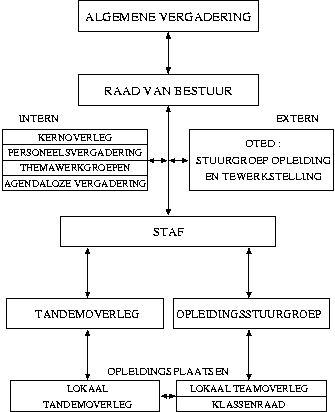
\includegraphics{../beeldjes/bewerkt/organogram.eps}
\clearpage% page: 1
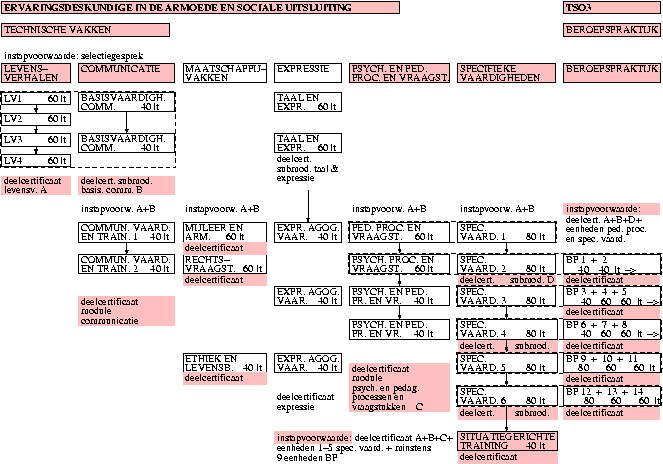
\includegraphics[%
  angle=270]{../beeldjes/bewerkt/opleidingsdiagram.eps}
\clearpage% page: 2
\includegraphics{../beeldjes/bewerkt/logo_deed.eps}
\clearpage% page: 3
\includegraphics{../beeldjes/bewerkt/attribution.eps}
\clearpage% page: 4
\includegraphics{../beeldjes/bewerkt/share-alike.eps}
\clearpage% page: 5
\includegraphics{../beeldjes/bewerkt/logo_code.eps}
\clearpage% page: 6

\end{document}
